\chapter{日常生活}

\section{工院人根据地}

自2023年新奥工学大楼建成以来，工学院各办公室、实验室陆续向燕东新园\footnote{即工学院、物理学院、城市与环境学院等院系所在的区域}迁移。目前，工学院在校内的分布集中在燕东新园的三栋楼内，即力学楼、工学院1号楼和新奥工学大楼。

\begin{figure}[htbp]
	\centering
	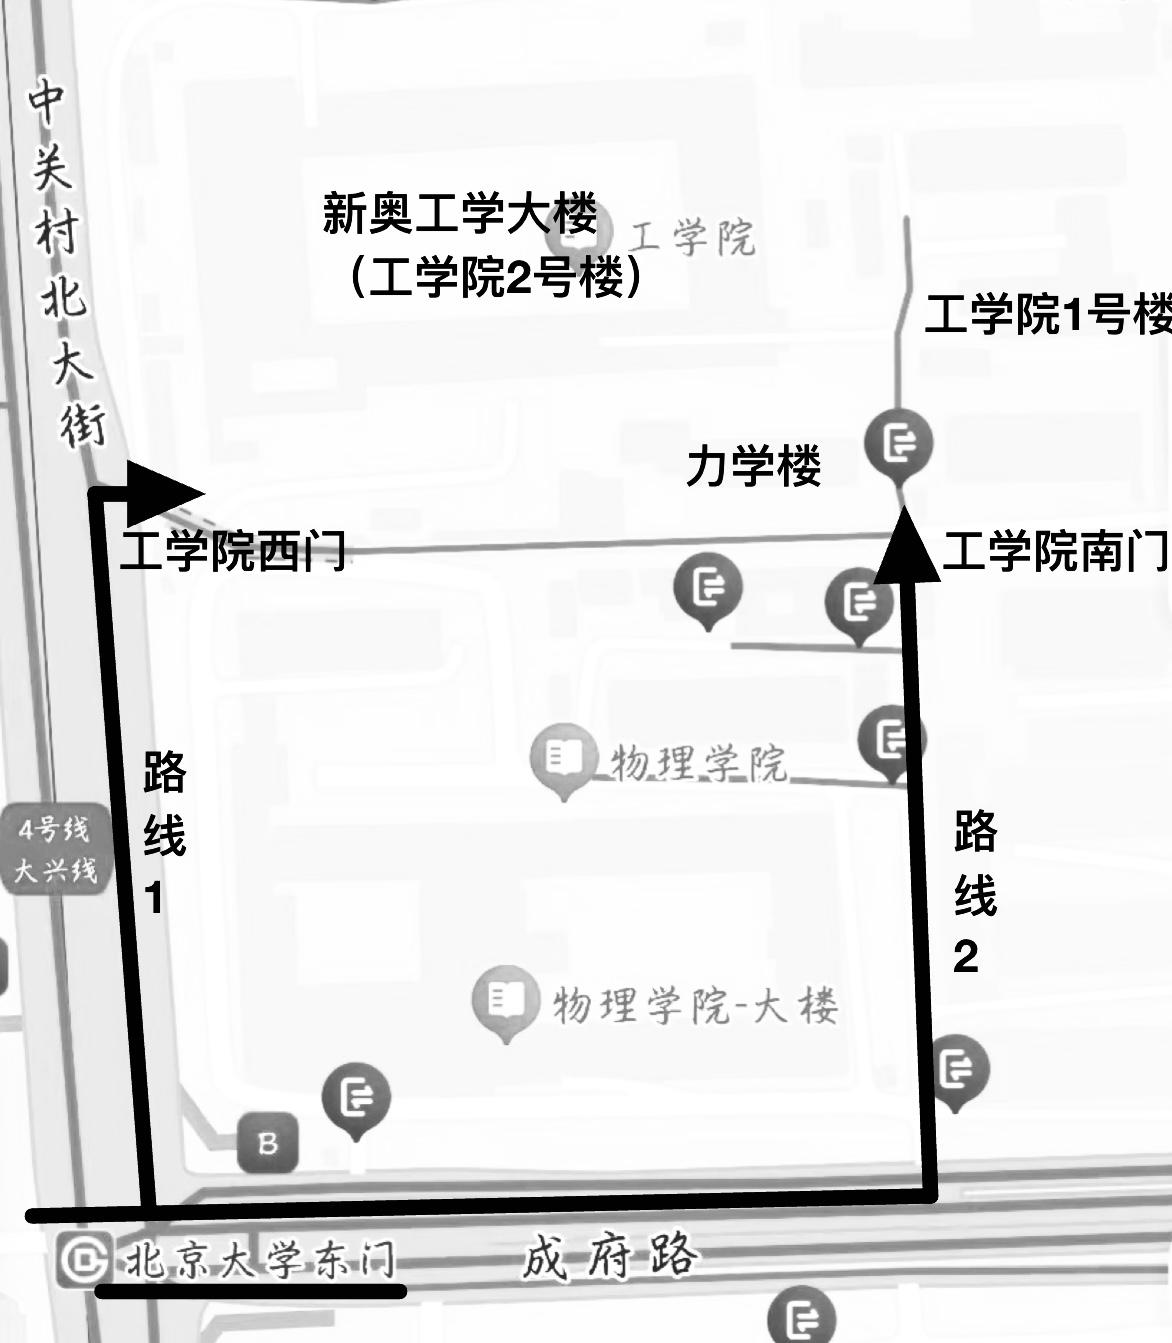
\includegraphics[width=0.5\linewidth]{assets/6.1工学大院地形.jpeg}
	\renewcommand{\figurename}{图}
	\caption{工学院主要建筑分布及通勤路径}
	\label{fig:enter-label}
\end{figure}

教务办公室、学生工作办公室均已搬入新奥工学大楼，分别位于2005室和2012室。负责其他事务的办公室位置也可进入工学院官网——办公服务——工学院办公室一栏查看。

\vspace{10pt}

需要提醒大家的是，老师们的办公室并非一定在新奥工学大楼内。故建议大家在与老师面谈前确认老师办公室所在地点。

\vspace{10pt}

工学院的三栋主要建筑内都有会议室。大多数情况下，学院内的大规模会议在这些地方举行：力学楼434，1号楼210，新奥工学大楼3004。

\vspace{10pt}

此外，燕南园60号也是工学院部分部门的办公地点，院子东北角立有写着“北京大学工学院”字样的石碑，是工学院新生打卡圣地。同学们通勤穿过燕南园时经常能路过60号院。

\vspace{10pt}

环境科学大楼（简称环境大楼）是北京大学环境科学与工程学院的教学科研大楼，大楼坐落于北京大学主校园的东北部成府园内，东临中关村北大街，毗邻微纳电子大厦、廖凯原楼（政府管理学院大楼）。

\vspace{10pt}

大楼集教学、科研、办公及学术交流于一体，包含地上五层，地下三层，房间编号是从西南角开始，逆时针方向连续编号。教学办公室（环境大楼104）与学生工作办公室（环境大楼212）位于大楼的一、二层，其余行政老师的办公室地点及联系方式可在“环境学院官网——师资队伍——行政人员”处进行查询。老师办公室与实验室主要位于大楼的三至五层，可在“师资队伍——在职教师”处查询老师们的办公地点与邮箱。

\vspace{10pt}

大楼负一层主要为会议室（B104、B110、B112、B121、B122、B130，以及一层的101室），会议室在无人使用时开放用作自习室，开放时间为8:00-23:00。

\vspace{10pt}

此外，大楼每层均设置有茶水间，并提供微波炉，有需要的同学可按照操作提示进行使用。

\section{信息渠道}
主动高效地获取、筛选信息，是每一位大学生的必修课。这门课优秀与否，在相当大的程度上决定了大家的学业水平和生活水平——某一门课的复习资料和往年题、诺奖得主的学术讲座、百讲的电影首映礼、校园十佳歌手决赛的门票领取……

\vspace{10pt}

进入大学，中学时代信息主动找上门的模式一去不复返，原地等待老师、学长学姐、同学、室友等他人告知的最终结局就是成为信息孤岛，错失关键大事。笔者曾耳闻某位同学四日未打开自己的校园邮箱，导致错失某关键奖项的申请——他本可以十拿九稳。此事虽是个例，却也足以说明主动掌握信息的重要性\footnote{以及每日检查邮箱的重要性！}。因此，我们建议大家充分利用各类渠道，尽快建立信息网络，将信息主动权掌握在自己手中。

\vspace{10pt}

在此，我们列出最为常用的各类渠道，以便大家日常使用，提高主动搜集、整理信息的能力。

\subsection{网站}

1. 北京大学信息门户\quad portal.pku.edu.cn

包含北大日常生活所需80\%的工具和信息，如校园卡（含充值、挂失等）、校园邮箱、校历、课表查询、成绩查询、体育场馆预约、访客预约、空闲教室查询、畅行清华等。同时有手机端APP，推荐大家安装，功能几乎相同，虽然界面适配仍待改进。

\vspace{10pt}

2. 北大树洞\quad treehole.pku.edu.cn

专属于北大人的匿名聊天平台。可查询数量极为庞大、内容极为丰富的民间信息，包括但不限于学习资料、课程评测、院系/专业体验、导师推荐、活动经验、生活技能、恋爱教程、美食攻略、旅游指南、跳蚤市场等。一言以蔽之：无数精彩内容等待大家探索！

需要注意的是，树洞上也有许多没有多少价值的内容，且发帖者（洞主）的立场和偏见、信息真假等均需自行辨别。此外，即使是匿名平台，也请大家务必注意遵守底线思维，不可发表违背公序良俗或法律法规的言论。

\vspace{10pt}

3. 北京大学教务部\quad dean.pku.edu.cn

包含北大有关课程、考试的种种信息，例如培养方案、选课退课、双专业/辅修、本科生科研等。任何学业、课程、政策等有关问题均可在该网站尝试搜索。

\vspace{10pt}

4. 北京大学选课网\quad elective.pku.edu.cn

顾名思义，选课期间最为重要的网站之一。选课网基本操作详见本手册2.3。

\vspace{10pt}

5. 北京大学教学网\quad course.pku.edu.cn

包含已选课程的相关信息，例如教师通知、课程回放、大纲、教案、作业、成绩\footnote{据笔者经验，只有少数课程成绩会在教学网上记录，大多数课程的成绩只出现在树洞上}等。

鉴于极具年代感的网页设计，笔者不得不向大家推荐一份专门美化教学网页面的插件：\\https://github.com/zhuozhiyongde/PKU-Art。具体下载、安装、使用方式，详见GitHub页面的详细说明。注意，笔者仅作推荐，不承担因使用该插件造成的任何损失。

\vspace{10pt}

6. 北京大学学生邮箱\quad mail.stu.pku.edu.cn 

稍正式沟通、交流的常用平台之一。学校或院系通知、活动项目、志愿者招募、师生交流等均会用到学生邮箱。需要注意的是，部分有价值的邮件可能会因判断机制被归入垃圾邮件，而不会出现在收件箱中。故在常规的收件箱之外，垃圾邮件亦需定期检查。

\vspace{10pt}

此处为大家透露一个小彩蛋：学校信息中心会不定期组织钓鱼邮件攻防演练，发送各类与大家学习、生活、兴趣等密切相关的模拟钓鱼邮件，“勾引”大家填写自己的学号和密码，随后跳转至“老师/同学，您已中招”的界面。笔者曾经历校园卡充值满减、端午节免费送粽子、新生情况有奖调查、免费试用Sora大模型等“勾引主题”。在提升诈骗防范能力的同时，笔者也不得不感慨信息中心花样真多（$\times$）。但是，认真地！大家作为新生，一定要提高防范意识，谨防网络诈骗！

\vspace{10pt}

7. 北京大学工学院\quad coe.pku.edu.cn

包含与工学院相关的信息、文件、新闻等，可查询各功能处室办公地址、奖学金评选通知、各专业培养方案、各系所教师队伍、各老师的研究方向和联系方式等。建议大家空闲时了解了解各位老师的研究方向，感兴趣的可以和老师多多交流，甚至可以进入老师的课题组，开启科研体验。早一些接触科研训练对本科生而言，总不是什么坏事。

\vspace{10pt}

8.北京大学环境学院\quad cese.pku.edu.cn

包含环境学院概况、教师信息、招生招聘信息，以及学院重大新闻等。

\vspace{10pt}

9. 北京大学信息中心\quad its.pku.edu.cn

校园网连接设备管理、网费充值、常见问题解决方案，正版软件（如Adobe系列、Microsoft Office、MATLAB等），邮箱使用指南等校园内一切有关“信息”的内容。

\vspace{10pt}

10.北大研招网\quad admission.pku.edu.cn

查询北大研究生招生、录取信息。

\vspace{10pt}

11.北大图书馆\quad www.lib.pku.edu.cn

提供北大图书馆图书借阅、研讨空间预约、活动/展览/讲座等信息。
	
\newpage

\subsection{公众号与小程序}

\[
\begin{matrix}
	\text{北京大学} & \text{公众号} & \text{正身自然不必多说}\\
	\text{工映青春} & \text{公众号} & \text{工学院学生活动信息平台，会发布一些重要通知}\\
	\text{北大体育} & \text{公众号} & \text{85km跑、五四跑、新生杯、北大杯等体育赛事通知}\\
	\text{PKU体委} & \text{公众号} & \text{85km跑相关通知，周二、周四夜奔点歌渠道}\\
	\text{赛艇先生} & \text{公众号} & \text{考试复习资料、往年题}\\
	\text{北大团委} & \text{公众号} & \text{团委活动通知，如中秋晚会、五四诗会等}\\
	\text{北京大学学生会} & \text{公众号} & \text{学生会活动通知，如十佳歌手、十佳主持人等}\\
	\text{P大CoE教务} & \text{公众号} & \text{工院教务公众号，发布学业、课程相关重要通知}\\
	\text{北京大学百周年纪念讲堂} & \text{公众号} & \text{电影、演出等信息}\\
	\text{北大与世界} & \text{公众号} & \text{对外交流项目相关信息}\\
	\text{北大就业} & \text{公众号} & \text{就业指导相关信息}\\
	\text{北大工学} & \text{公众号} & \text{工学院新闻、学术、科研等通知}\\
	\text{北大环院} & \text{公众号} & \text{环境学院最新动态与新闻}\\
	\text{北大环院人} & \text{公众号} & \text{团委、学生会、研会信息发布、活动宣传与风采展示平台}\\
	\text{北京大学学生发展支持} & \text{公众号} & \text{学业辅导、生涯规划等方面的支持}\\
	\text{北大餐饮中心官方资讯} & \text{公众号} & \text{食堂、菜品、特色美食信息}\\
	\text{北京大学图书馆} & \text{小程序} & \text{馆藏内容检索、云打印服务等}\\
	\text{北大空间} & \text{小程序} & \text{预约空闲教室用于自习等}\\
	\text{志愿北京} & \text{小程序} & \text{查看志愿服务学时}\\
	\text{北大文创} & \text{小程序} & \text{文创产品的线上购买、邮寄等}\\
	\text{动力中心收费服务号} & \text{小程序} & \text{查询宿舍用电购电情况，及时充值缴费购电}\\
	\text{燕园学子微助手} & \text{小程序} & \text{北京大学学生工作部发布校园活动宣传推送}\\
\end{matrix}
\]

\subsection{软件}

1. 北京大学APP

与北大门户网站功能相似。

\vspace{10pt}

2. bilibili

无数宝藏课程的荟萃地，同时也是娱乐的天堂。

\vspace{10pt}

3. MATLAB

工学院必备，但大一用处不算大，可提前学习掌握。

\vspace{10pt}

4. 各类IDE软件

IDE（Integrated Development Environment），集成开发环境。用于编写代码，

如Visual Studio Code、PyCharm、Spider、Dev C++等，具体可咨询计算机课程老师或助教，自行比较择优即可。

\vspace{10pt}

5. 手写笔记软件

Goodnotes、Notability、Notein一笔记等，用于手写笔记、绘图等。笔者自觉好用的（例如上述三者）均需付费\footnote{提醒：切勿相信各类低价Goodnotes/Notability账号信息，笔者曾购买所谓永久账号，使用了三周便被封禁（悲）。擦亮双眼，不贪小便宜！}。注意：定期备份！毕竟谁也不想看到软件bug让辛辛苦苦写了一学期的数分笔记在期末周灰飞烟灭。

\subsection{校内联系电话}

\textbf{·保卫部：62755110}

\textbf{·燕园派出所：62751331}

生病、受伤等无法自主行动时，可拨打保卫部电话，前往校医院。

\vspace{10pt}

\textbf{·心理咨询中心：62760852}

\textbf{·24小时心理援助热线：62760521}

情绪没有对错，困难不必独行。笔者真诚地希望你在逐梦的路上，也能照顾好自己的心灵。

\vspace{10pt}

\textbf{·校医院：62759011}

\textbf{·校医院24小时急诊电话：62751919}

\vspace{10pt}

\textbf{·勺园酒店：62752218，62757361，62752200}

\textbf{·中关新园：62755236}

若大家有同学、亲友到访且需住宿，可通过上述电话联系酒店预定房间。持学生卡预定可享受优惠。
